\chapter{Implementación}

Neste capítulo se comentarán os aspectos máis relevantes da implementación da nosa plataforma.


\section{Servidor}
Spring en todo o proxecto
Autenticación con Google: Só facer mención á sección posterior
ASWS.

\subsection{Acceso á base de datos}
Exemplo de acceso a datos

\subsection{Construción dos servizos web}
Exemplo de construción dos servizos web: Spring MVC












\subsection{Transaccionalidade}
A xestión transaccionalidade impleméntase na capa Manager utilizando o framework Spring, grazas á súa librería spring-tx. A súa configuración e utilización é moi sinxela, tal e como se pode observar nos exemplos. No primeiro amósase a configuración que require nos ficheiros XML de Spring. Para indicar a transaccionalidade, utilizaremos etiquetas que permitan identificar o tipo de transacción que queremos que se aplique en cada método público do manager. Non todos os métodos provocan escrituras en base de datos, polo que non será necesario indicar o tipo de transaccionalidade que provoca desfacer cambios en todos eles. O resto marcaranse como de só lectura para non sobrecargar innecesariamente o sistema.

Na figura~\ref{fig:transaccionConfiguracion} pódese observar a configuración da transaccionalidade nos ficheiros XML.

\begin{figure}[tbh] 
	\begin{center}
		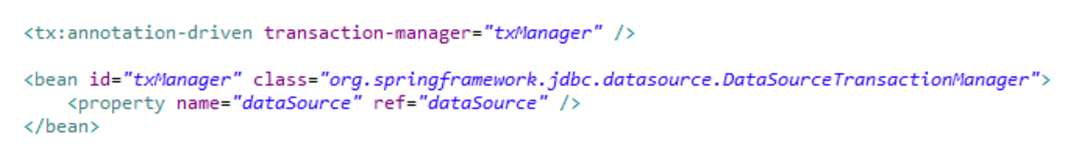
\includegraphics[width=1\textwidth]{figures/codigo/transaccionConfiguracion}
		\caption{Configuración da transaccionalidade no ficheiro XML.}
		\label{fig:transaccionConfiguracion}
	\end{center}
\end{figure}


Na figura~\ref{fig:metodoTransaccional} pódese observar a configuración da transaccionalidade sobre un método no que se modifican datos.

\begin{figure}[tbh] 
	\begin{center}
		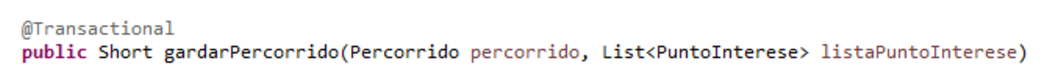
\includegraphics[width=1\textwidth]{figures/codigo/metodoTransaccional}
		\caption{Configuración da transaccionalidade dun método onde se modifican datos.}
		\label{fig:metodoTransaccional}
	\end{center}
\end{figure}

Na figura~\ref{fig:metodoNonTransaccional} pódese observar a configuración da transaccionalidade sobre un método de só lectura.

\begin{figure}[tbh] 
	\begin{center}
		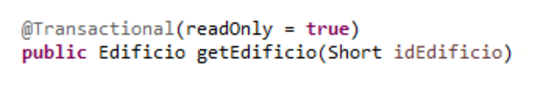
\includegraphics[width=0.5\textwidth]{figures/codigo/metodoNonTransaccional}
		\caption{Configuración da transaccionalidade dun método de só lectura.}
		\label{fig:metodoNonTransaccional}
	\end{center}
\end{figure}


\section{Aplicación Android}

\subsection{Solicitude de permisos}
Como se solicitan permisos na aplicación
Non fan falla na instalación. Solicítanse na execución. Sen o permiso de localización non funcionaría a aplicación.

\subsection{Acceso a Situm}
Exemplo de acceso a Situm

\subsection{Acceso ao servidor}
Exemplo de acceso ao servizo web




Exemplo de chamada a actividade e devolución do fluxo

Para publicar a aplicación na Play Store
https://developer.android.com/studio/publish/app-signing




\section{Autenticación}

https://developers.google.com/identity/sign-in/android/start-integrating


https://developers.google.com/android/guides/client-auth


Incluír o google-services.json dentro da aplicación Android para permitir a conexión